% Method schematic (version 3): one flow, top to bottom, ALL positions relative.
% Compile standalone from the manuscript folder:  pdflatex method_schematic3.tex
% (loads ../figure/fig3.png for the municipality map)
%
% HOW TO MOVE THINGS
%  * every plot is a named node `parea` (size \pw x \ph cm); curves are drawn in the
%    plot's own local coordinates (0..\pw, 0..\ph), so they follow the node.
%  * to move a plot: edit its `at ([shift={(dx,dy)}]othernode)` / `below=..of` line.
%  * to resize all plots: change \pw / \ph (curves rescale automatically).
\documentclass[tikz,border=6pt]{standalone}
\usepackage{amsmath}
\usepackage{graphicx}
\usetikzlibrary{arrows.meta,calc,positioning,fit,backgrounds,shapes.misc}
\pgfdeclarelayer{bottom}   % below `background`: for the overall frame
\pgfsetlayers{bottom,background,main}

\usepackage[scaled]{helvet}
\renewcommand{\familydefault}{\sfdefault}

\definecolor{tNavy}{HTML}{1A3B5D}
\definecolor{tTeal}{HTML}{1B9E77}
\definecolor{tOrng}{HTML}{E6550D}
\definecolor{cZur}{HTML}{0057B8}   % Zurich  (same as the map)
\definecolor{cGen}{HTML}{009E73}   % Geneva
\definecolor{cBas}{HTML}{7B3294}   % Basel
\definecolor{pFill}{HTML}{FBFCFE}
\definecolor{pEdge}{HTML}{C7D2E0}
\definecolor{yFill}{HTML}{FFFDF4}   % (unused now) pale yellow
\definecolor{rFill}{HTML}{FFF7F5}   % very light red    : national level boxes
\definecolor{rEdge}{HTML}{F3D8D4}
\definecolor{vFill}{HTML}{F8F5FC}   % very light violet : municipal level boxes
\definecolor{vEdge}{HTML}{DDD3EC}
\definecolor{yEdge}{HTML}{F3EBC9}
\definecolor{cA15}{HTML}{F2A65A}   % light orange
\definecolor{cA50}{HTML}{9E2B25}   % dark red
\definecolor{cFd}{HTML}{15497A}    % fertility : dark blue
\definecolor{cFl}{HTML}{7FB3E0}    % fertility : light blue

% ------------------------------------------------------------------ parameters
\def\pw{2.2}     % plot width  (cm)
\def\ph{1.2}   % plot height (cm)
\def\cfdx{0.75}   % cm: gap between Expected births and its text box (bigger = further right)
\def\cfdy{0.9}   % cm: how far the Expected-birth text box is raised
\def\bgap{0.6}   % cm: horizontal gap between Shift | Season | Trend (min ~0.6: y labels)
\def\nbgap{1.5} % vertical gap (cm) between the model box and National births (above it)
\def\popdx{2.2}   % cm: Population plot centre is this far LEFT of the model box's left edge
\def\nexph{1.6}   % cm: height of the National excess plot (bigger than \ph); Municipality-level box copies its box size
\def\jdy{0.7}    % cm: height above National excess where the two arrows join
\def\adx{0.7cm}   % off-centre arrows lean toward the middle of the figure by this much
\def\nedy{1.7}  % cm: model box -> National expectation (room for the three arrows)
\def\rowdy{2.1} % cm: National expectation -> row of National excess / Municipality-level
\def\mexdy{2.2} % cm: Municipality-level -> Municipal excess/deficit
\def\agap{6pt}  % vertical gap left at the start/end of arrows (same y for all arrows)
\def\tgap{0pt}  % gap between a plot and its title (national excess uses 3pt)

% plot decoration: axes + title + x label + y label, attached to node #1.
% optional first argument = how far left the y label sits (default 2pt)
\newcommand{\pdeco}[5][2pt]{%
  \draw[ax] (#2.south west)--(#2.south east);
  \draw[ax] (#2.south west)--(#2.north west);
  \node[ttl,anchor=south] (#2-t) at ([yshift=\tgap]#2.north) {#3};
  \node[sub,anchor=north] (#2-x) at ([yshift=-1pt]#2.south) {#4};
  \node[sub,rotate=90,anchor=south] (#2-y) at ([xshift=-#1]#2.west) {#5};
}

\begin{document}
\begin{tikzpicture}[
  font=\sffamily,
  >={Stealth[length=8pt,width=6pt]},
  panel/.style={draw=pEdge,fill=pFill,rounded corners=4pt,line width=.9pt},
  box/.style={draw=pEdge,fill=white,rounded corners=3pt,line width=.7pt},
  parea/.style={minimum width=\pw cm,minimum height=\ph cm,inner sep=0pt,outer sep=0pt},
  ttl/.style={font=\fontsize{6}{7}\selectfont\bfseries,text=tNavy},   % plot titles
  sub/.style={font=\fontsize{4.5}{5}\selectfont,text=black!60},   % axis titles
  ax/.style={black!45,line width=.5pt},
  zero/.style={black!50,line width=.5pt,densely dashed},
  a50/.style={draw=cA50,line width=1pt},
  fdk/.style={draw=cFd,line width=1pt},
  flt/.style={draw=cFl,line width=1pt},
  agg/.style={draw=cA15!50!cA50,line width=1pt},   % mix of the two age colours
  flow/.style={->,draw=black!55,line width=1pt,},
]

% ====================================================================
% 3. Big box with three plots: Shift in childbearing age | Trend | Season
% ====================================================================
\node[parea] (tr) at (0,0) {};              % middle plot (Trend) = origin of the figure
\node[parea,left =\bgap cm of tr] (sh) {};   % Shift (left)
\node[parea,right=\bgap cm of tr] (se) {};   % Season (right)

\pdeco{tr}{Trend}{Time}{Birth rate}
\pdeco{se}{Season}{Time}{Birth rate}
\pdeco{sh}{Shift in childbearing age}{Age}{Fertility}

% trend: straight decreasing line
\begin{scope}[shift={(tr.south west)}]
  \draw[a50] (0.05,1.2)--(\pw-0.05,0.35);
\end{scope}
% season: seasonal sine (3 seasons), no trend
\begin{scope}[shift={(se.south west)}]
  \draw[a50] plot[domain=0.05:\pw-0.05,samples=100,smooth]
    (\x,{0.75+0.3*sin(3*\x/\pw*360)});
\end{scope}
% shift in childbearing age: same fertility curve, shifted horizontally
% (centres/width are fractions of \pw, so both curves always fit entirely in the plot)
\begin{scope}[shift={(sh.south west)}]
  \draw[fdk] plot[domain=0.05:\pw-0.05,samples=80,smooth]
    (\x,{0.1+1.1*exp(-((\x-0.364*\pw)/(0.164*\pw))*((\x-0.364*\pw)/(0.164*\pw)))});
  \draw[flt] plot[domain=0.05:\pw-0.05,samples=80,smooth]
    (\x,{0.1+1.1*exp(-((\x-0.636*\pw)/(0.164*\pw))*((\x-0.636*\pw)/(0.164*\pw)))});
\end{scope}

% the big box wraps the three plots and their labels
\coordinate (bbR) at ($(tr)!-1!(sh-y.north |- tr)$);   % mirror image of the left edge -> box is symmetric about Trend
\begin{scope}[on background layer]
  \node[panel,fill=rFill,draw=rEdge,fit=(bbR)(sh-y)(sh-t)(sh-x)(se-t)(se-x)(tr-t)(tr-x)(tr),inner xsep=7pt,inner ysep=3pt] (bigbox) {};
\end{scope}

% ====================================================================
% 1. National births (top, centred)
% ====================================================================
\node[parea,anchor=south] (nb) at ($(bigbox.north)+(0,\nbgap cm)$) {};   % centred exactly above the model box
\pdeco{nb}{Observed births}{Time}{Births}
\begin{scope}[shift={(nb.south west)}]
  \draw[a50] plot[domain=0.05:\pw-0.05,samples=100,smooth]
    (\x,{0.55+0.17*\x+0.14*sin(3*\x/\pw*360)});
\end{scope}

% ====================================================================
% 4. Expected births (centred under the model box, i.e. under Observed births) + text box on its right
% ====================================================================
\node[parea,anchor=north] (ne) at ($(bigbox.south)+(0,-\nedy cm)$) {};   % same centre line as Observed births
\pdeco{ne}{Expected births}{Time}{Births}
\begin{scope}[shift={(ne.south west)}]
  % expected line only
  \draw[agg,dashed] plot[domain=0.05:\pw-0.05,samples=100,smooth]
    (\x,{0.95-0.1*\x+0.11*sin(3*\x/\pw*360)});
\end{scope}

% ====================================================================
% 2. Population: small plot on the LEFT of the model box, level with it
% ====================================================================
\def\ppw{1.7}   % population plot width  (cm)
\def\pph{0.9}   % population plot height (cm)
\node[parea,minimum width=\ppw cm,minimum height=\pph cm] (pop) at ($(bigbox.west |- bigbox.center)+(-\popdx cm,0)$) {};
\pdeco{pop}{Population}{Time}{Pop. size}
\begin{scope}[shift={(pop.south west)},xscale={\ppw/\pw},yscale={\pph/\ph}]
  \draw[a50] (0.05,0.35) .. controls (1,0.5) and (2,0.8) .. (\pw-0.05,1.1);
\end{scope}

\node[box,draw=none,fill=black!6,rounded corners=0pt,text width=2.7cm,align=left,font=\fontsize{5}{6}\selectfont,inner sep=4pt,right=\cfdx cm of ne,yshift=\cfdy cm] (cf)
  {\textbf{Expected birth}: Counterfactual number of birth given\\[2pt]
   $\bullet$~a \textbf{stable} birth rate (i.e., no trend)\\
   $\bullet$~the population changes\\
   $\bullet$~shift in childbearing age\\
   $\bullet$~seasonal variation};



% ====================================================================
% 5. National excess/deficit (below, a bit right)  and  Municipality-level map (below, a bit left)
%    both are hung from the same row y, so their titles are at the same height
% ====================================================================
\coordinate (row2) at ($(nb |- ne-x.south)+(0,-\rowdy cm)$);   % lower row stays centred on National births
\node[parea,anchor=north,minimum height=\nexph cm] (nex) at ([xshift=2.4cm]row2) {};
\def\tgap{3pt}\pdeco[9pt]{nex}{National excess/deficit of births}{Time}{Excess/deficit}\def\tgap{1pt}
\begin{scope}[shift={(nex.south west)},yscale={\nexph/\ph}]
  \def\obsx{0.7875-0.0583*\x+0.14*sin(3*\x/\pw*360)}      % observed
  \def\expx{0.6125+0.0583*\x+0.11*sin(3*\x/\pw*360)}      % expected
  \draw[zero] (0,{\ph/2})--(\pw,{\ph/2});
  \node[sub,anchor=east] at (0,{\ph/2}) {0};
  % excess/deficit = observed - expected (x2.5 for visibility)
  \draw[agg] plot[domain=0.05:\pw-0.05,samples=100,smooth]
    (\x,{\ph/2+2.5*((\obsx)-(\expx))});
\end{scope}
% its box, drawn now so that the Municipality-level box can copy its size
\begin{scope}[on background layer]
  \coordinate (nex-yr) at ($(nex)!-1!(nex-y.north |- nex)$);
  \node[box,fill=rFill,draw=rEdge,fit=(nex-yr)(nex-y)(nex-t)(nex-x)(nex),inner sep=3pt] (nex-box) {};
\end{scope}
% measure that box (width, height) and the height of a title, in pt
\path let \p1=($(nex-box.north east)-(nex-box.south west)$) in \pgfextra{\xdef\nexw{\x1}\xdef\nexh{\y1}};
\path let \p1=($(nex-t.north)-(nex-t.south)$) in \pgfextra{\xdef\ttlh{\y1}};
\pgfmathsetlengthmacro{\imgh}{\nexh-6pt-\ttlh-1pt}   % map height so that the box height = National excess box height

% municipality-level map, box = same size as the National excess box
\node[inner sep=0pt,anchor=north] (mun) at ([xshift=-2.4cm,yshift=2pt]row2)
  {\IfFileExists{../figure/fig_expected_births_map.png}%
    {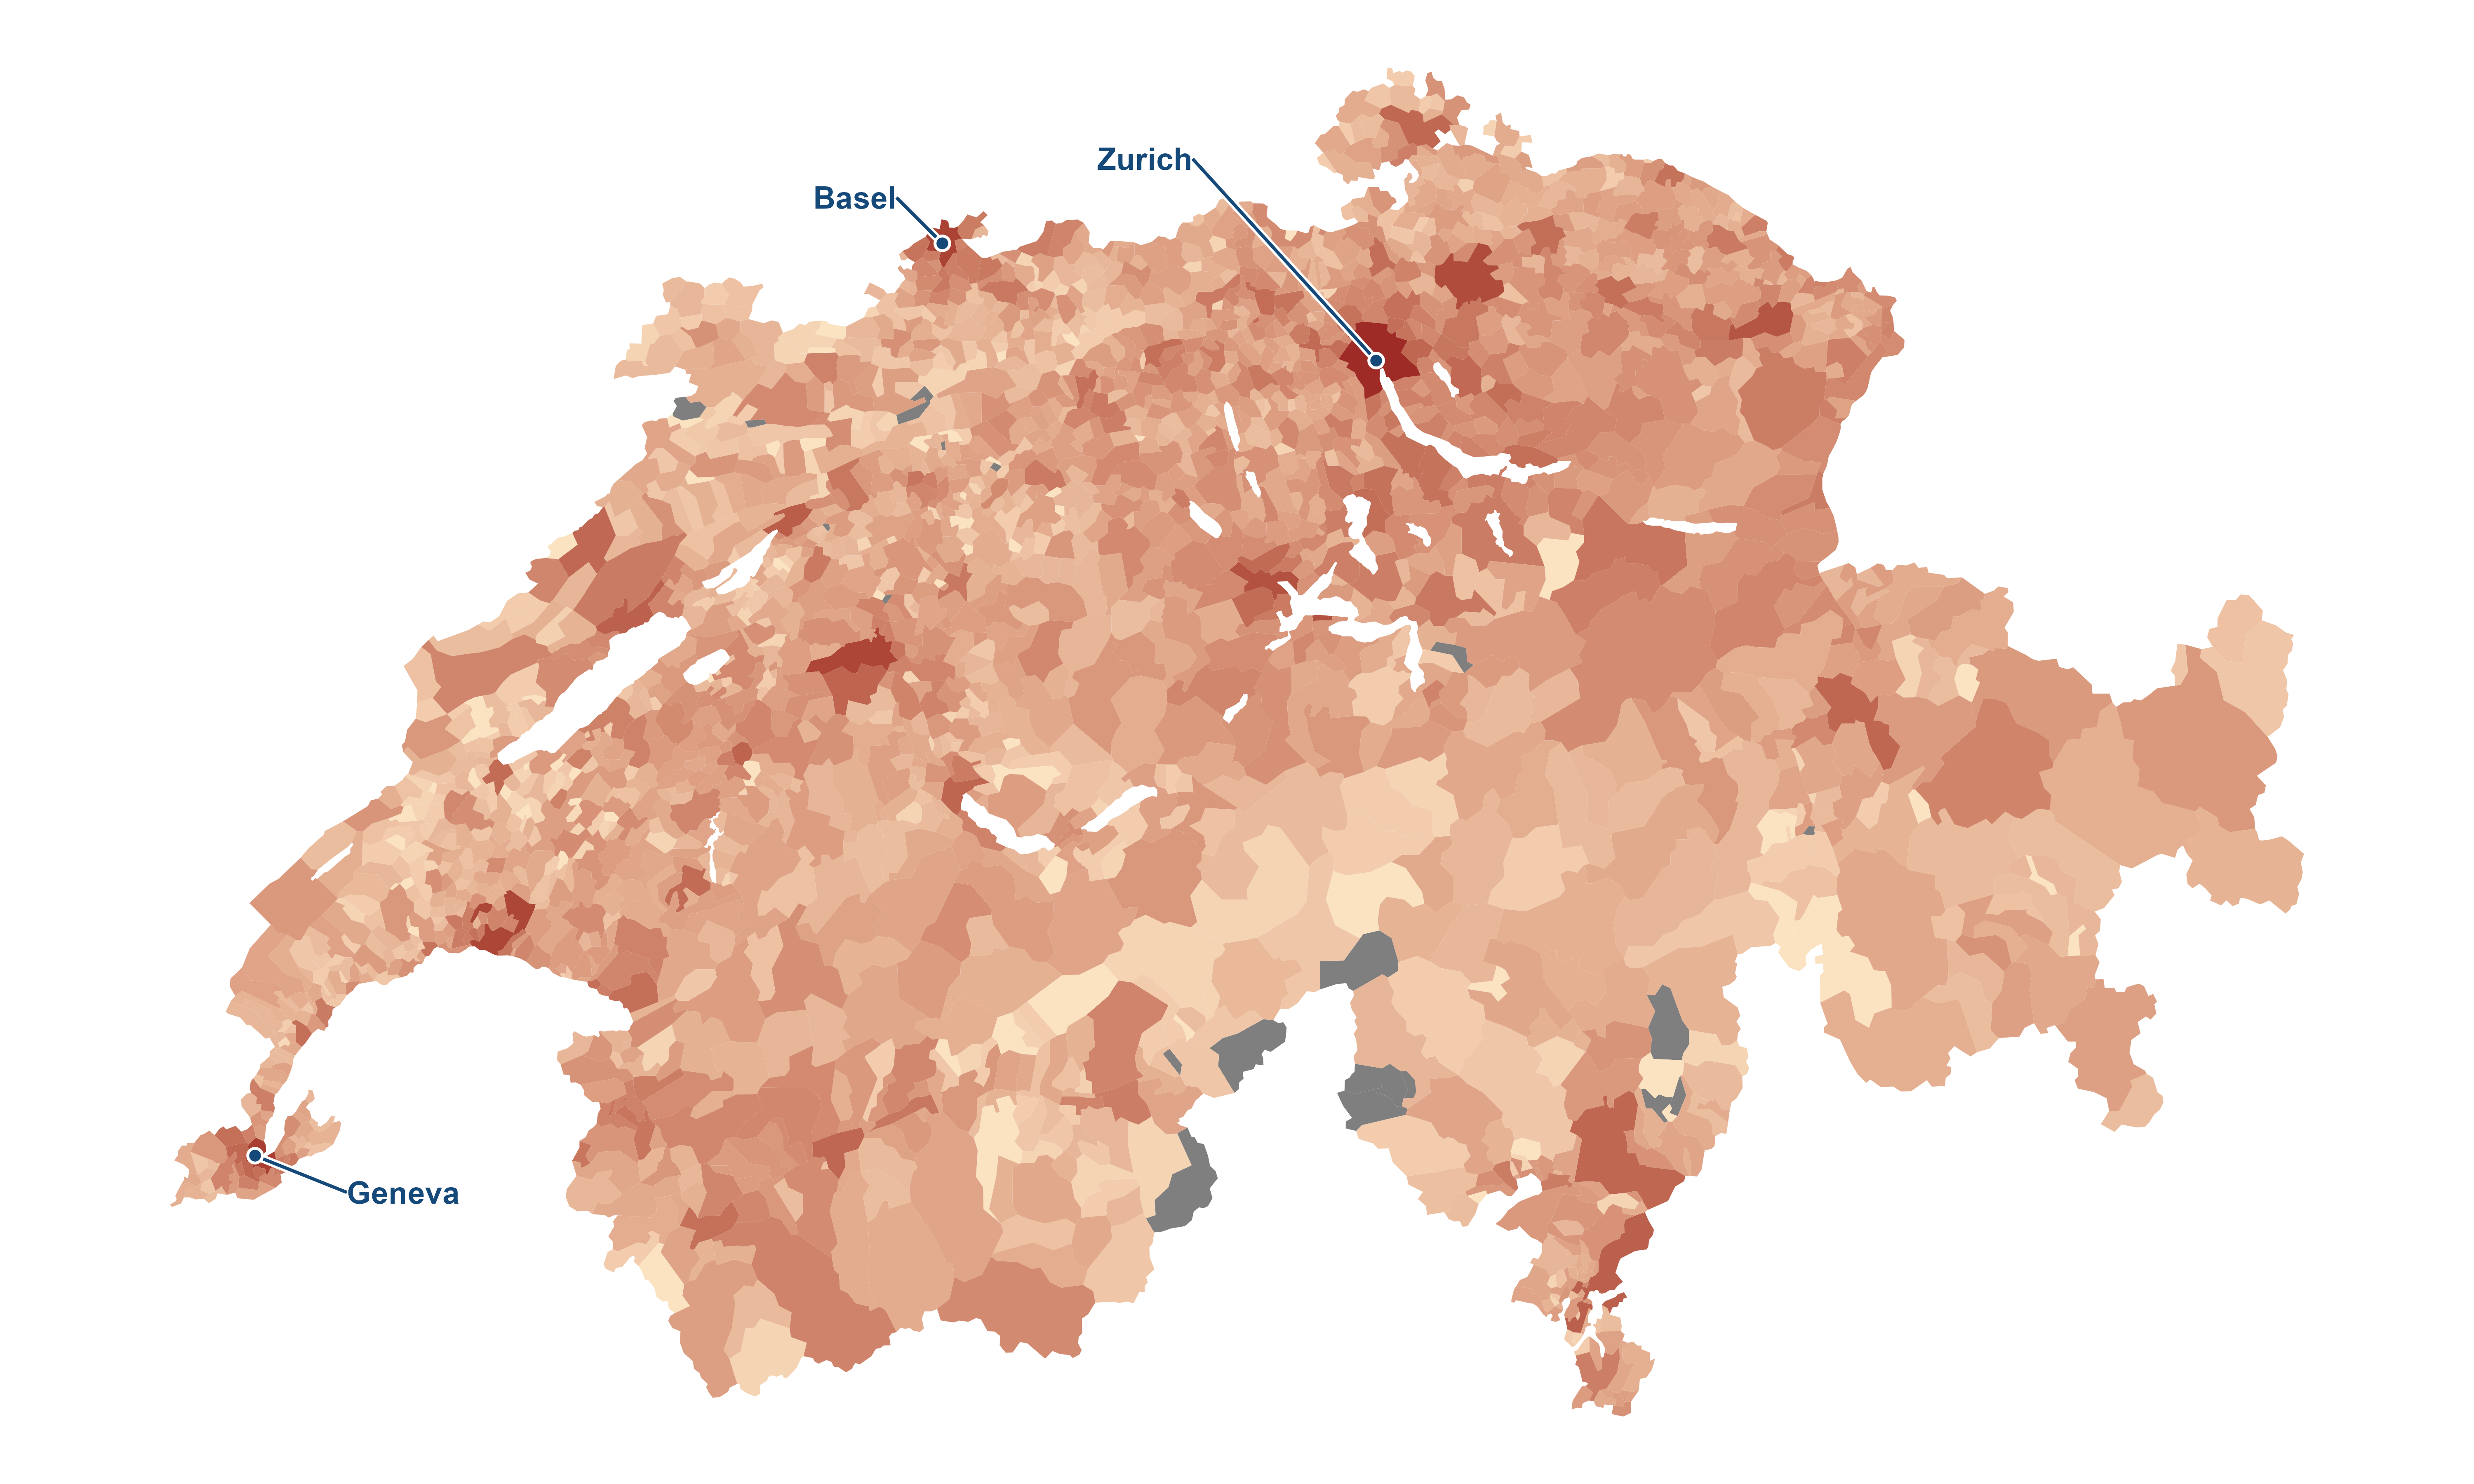
\includegraphics[height=\imgh]{../figure/fig_expected_births_map.png}}%   expected births 2025 (run reports/fig_expected_births_map.R)
    {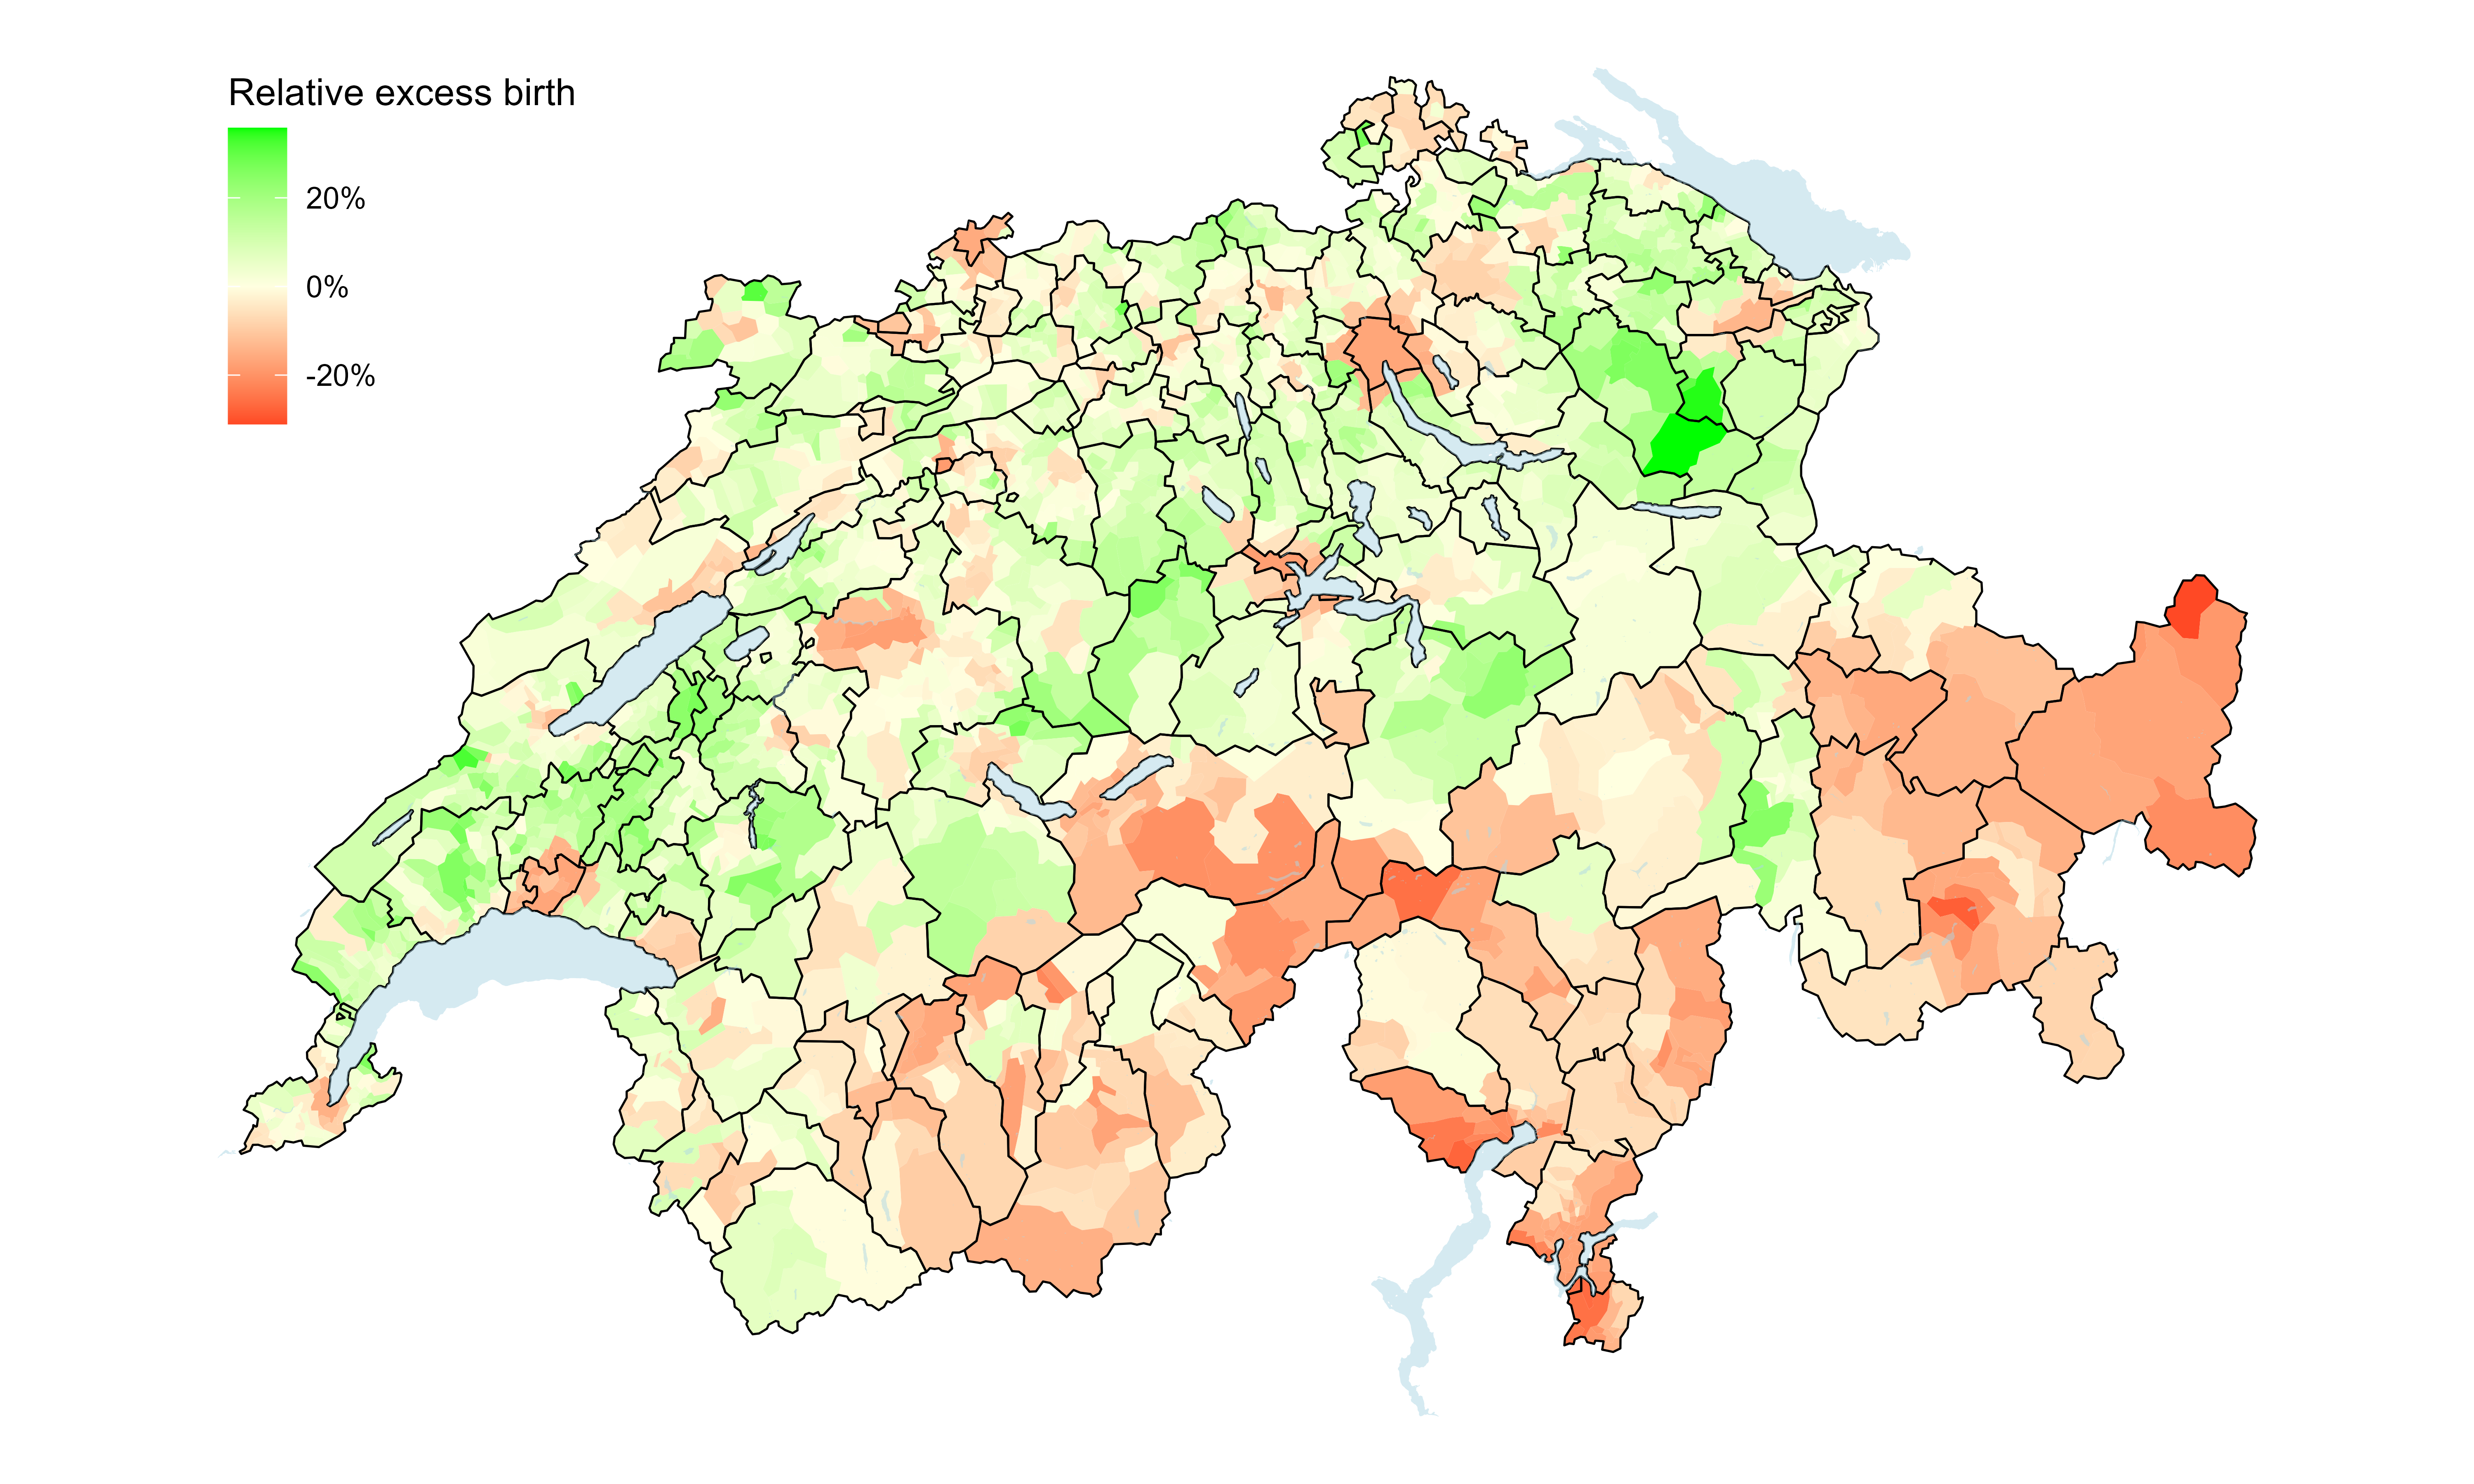
\includegraphics[height=\imgh]{../figure/fig3.png}}};   % fallback until that file exists
\node[ttl,anchor=south] (mun-t) at ([yshift=1pt]mun.north) {Municipality-level};
\begin{scope}[on background layer]
  \node[box,fill=vFill,draw=vEdge,fit=(mun-t)(mun),inner sep=3pt,minimum width=\nexw] (mun-box) {};
\end{scope}


% ====================================================================
% 6. Municipal excess/deficit (below the municipality map), two coloured lines
% ====================================================================
\node[parea,below=\mexdy cm of mun] (mex) {};
\pdeco[9pt]{mex}{Municipal excess/deficit of births}{Time}{Excess/deficit}
\begin{scope}[shift={(mex.south west)}]
  \draw[zero] (0,{\ph/2})--(\pw,{\ph/2});
  \node[sub,anchor=east] at (0,{\ph/2}) {0};
  % three curves = the three biggest cities (colours as on the map)
  \draw[draw=cZur,line width=1pt] plot[domain=0.05:\pw-0.05,samples=100,smooth]
    (\x,{\ph/2+0.4-0.27*\x+0.07*sin(3*\x/\pw*360)});
  \draw[draw=cGen,line width=1pt] plot[domain=0.05:\pw-0.05,samples=100,smooth]
    (\x,{\ph/2-0.25+0.12*\x+0.07*sin(3*\x/\pw*360+60)});
  \draw[draw=cBas,line width=1pt] plot[domain=0.05:\pw-0.05,samples=100,smooth]
    (\x,{\ph/2+0.08-0.04*\x+0.07*sin(3*\x/\pw*360+120)});
\end{scope}


% ====================================================================
% boxes around single plots (title + axis labels included). Add/remove a line to toggle one.
% ====================================================================
% national-level boxes: very light red (Population)
\foreach \n in {pop}{
  \begin{scope}[on background layer]
    \coordinate (\n-yr) at ($(\n)!-1!(\n-y.north |- \n)$);
    \node[box,fill=rFill,draw=rEdge,fit=(\n-yr)(\n-y)(\n-t)(\n-x)(\n),inner sep=3pt] (\n-box) {};
  \end{scope}
}
% municipal-level box: very light violet (Municipal excess/deficit)
\foreach \n in {mex}{
  \begin{scope}[on background layer]
    \coordinate (\n-yr) at ($(\n)!-1!(\n-y.north |- \n)$);
    \node[box,fill=vFill,draw=vEdge,fit=(\n-yr)(\n-y)(\n-t)(\n-x)(\n),inner sep=3pt] (\n-box) {};
  \end{scope}
}

% observed births and expected births: very light red
\foreach \n in {nb,ne}{
  \begin{scope}[on background layer]
    \coordinate (\n-yr) at ($(\n)!-1!(\n-y.north |- \n)$);
    \node[box,fill=rFill,draw=rEdge,fit=(\n-yr)(\n-y)(\n-t)(\n-x)(\n),inner sep=3pt] (\n-box) {};
  \end{scope}
}


% ====================================================================
% ARROWS -- every arrow is defined from the EDGES of the boxes (nb-box, pop-box, bigbox,
% ne-box, cf, nex-box, mun-box, mex-box). \agap = clear space left at each end.
% Off-centre arrows lean toward the middle of the figure by \adx.
% ====================================================================
% box title: ABOVE the model box, left-aligned with it
\node[ttl,anchor=south west] (bb-t) at ($(bigbox.north west)+(0,2pt)$) {Model decomposition};

% national (observed) births -> model box, centre
\draw[flow] ($(nb-box.south)+(0,-\agap)$) -- ($(bigbox.north)+(0,\agap)$);   % straight, centre to centre
% italic comment on the right of that arrow, two lines (width-limited)
\node[anchor=west,inner sep=0pt,align=left,text width=1.6cm,font=\tiny\itshape,text=black!65]
  at ($($(nb-box.south)+(0,-\agap)$)!0.5!($(bigbox.north)+(0,\agap)$)+(2pt,0)$) {inferred by the Bayesian model};

% shift (left), trend (middle, faded + red cross), season (right) -> expected births.
% All three start on the SAME y (bottom edge of the model box) and end on the SAME y.
% Shift and Season arrows are exact mirror images about the centre line.
\coordinate (sL) at ($(sh.south |- bigbox.south)+(\adx,-\agap)$);    % Shift  (left)
\coordinate (sM) at ($(tr.south |- bigbox.south)+(0,-\agap)$);        % Trend  (middle)
\coordinate (sR) at ($(se.south |- bigbox.south)+(-\adx,-\agap)$);   % Season (right)
\coordinate (neL) at ($(ne-box.north)+(-0.6cm,\agap)$);
\coordinate (neM) at ($(ne-box.north)+(0,\agap)$);
\coordinate (neR) at ($(ne-box.north)+(0.6cm,\agap)$);
\draw[flow] (sL) -- (neL);
\draw[flow,opacity=.4] (sM) -- (neM);   % trend: faded + crossed
\draw[flow] (sR) -- (neR);
\node[cross out,draw=red,line width=1.8pt,minimum size=0.3cm,inner sep=0pt]
  at ($(sM)!0.5!(neM)$) {};

% population -> model box: horizontal, right middle of Population to the left side of the model box
\draw[flow] ($(pop-box.east)+(\agap,0)$) -- ($(pop-box.east -| bigbox.west)+(-\agap,0)$);
% population -> expected births: down from the bottom of Population, then right into Expected births
\draw[flow,rounded corners=8pt] ($(pop-box.south)+(0,-\agap)$) |- ($(ne-box.west)+(-\agap,0)$);

% observed births -> national excess/deficit: out to the right, down the right of the
% model box / text box (routeR), then left into the box
\coordinate (routeR) at ($(bigbox.east)+(0.4cm,0)$);   % vertical run: clear of the model box (and the text box)
\coordinate (nexE) at ($(nex-box.north)+(-\adx,\agap)$);   % common arrival point on National excess/deficit
\coordinate (nexJ) at ($(nexE)+(0,\jdy cm)$);   % the two arrows JOIN here, then one short arrow goes down to nexE
\coordinate (oS) at ($(nb-box.east)+(\agap,0)$);
% horizontal -> vertical -> diagonal: (obsP) is where the vertical run ends and the diagonal starts
\coordinate (obsP) at ($(routeR |- nexJ)+(0,0.5cm)$);   % 0.5cm = height of the diagonal part
\draw[flow,-,rounded corners=8pt] (oS) -- (oS -| routeR) -- (obsP) -- (nexJ);   % no head: it joins the other arrow
\draw[flow] (nexJ) -- (nexE);                                  % common final arrow

% expected births -> national / municipality-level
\draw[flow,-] ($(ne-box.south)+(0.4cm,-\agap)$)  -- (nexJ);
% comment on the common final arrow: right of it, just before it arrives, two lines (width-limited)
\node[anchor=west,inner sep=0pt,align=left,text width=1.4cm,font=\tiny\itshape,text=black!65]
  at ($(nexJ)!0.5!(nexE)+(2pt,0)$) {compared to observed births};
\draw[flow] ($(ne-box.south)+(-0.4cm,-\agap)$) -- ($(mun-box.north)+(\adx,\agap)$);

% municipality-level -> municipal excess/deficit (same centre line)
\draw[flow] ($(mun-box.south)+(0,-\agap)$) -- ($(mex-box.north)+(0,\agap)$);   % same centre line: straight

% ====================================================================
% 7. Municipal data boxes (left column, same kind as Population)
% ====================================================================
% (a) Municipal population: level with the MIDDLE of the arrow Expected births -> Municipality-level;
%     horizontal dashed line from its right middle to that midpoint
\coordinate (m1a) at ($(ne-box.south)+(-0.4cm,-\agap)$);
\coordinate (m1b) at ($(mun-box.north)+(\adx,\agap)$);
\coordinate (M1) at ($(m1a)!0.5!(m1b)$);                % middle of that arrow
\node[parea,minimum width=\ppw cm,minimum height=\pph cm] (mp) at (pop |- M1) {};
\pdeco{mp}{Municipal population}{Time}{Pop. size}
\begin{scope}[shift={(mp.south west)},xscale={\ppw/\pw},yscale={\pph/\ph}]
  % three curves = the three biggest cities (colours as on the map and in Municipal excess)
  \draw[draw=cZur,line width=1pt] (0.05,0.75) .. controls (1,0.85) and (2,0.95) .. (\pw-0.05,1.1);
  \draw[draw=cGen,line width=1pt] (0.05,0.5)  .. controls (1,0.55) and (2,0.5)  .. (\pw-0.05,0.45);
  \draw[draw=cBas,line width=1pt] (0.05,0.25) .. controls (1,0.3)  and (2,0.4)  .. (\pw-0.05,0.6);
\end{scope}
% (b) Municipal births: level with the MIDDLE of the arrow Municipality-level -> Municipal excess;
%     straight horizontal line (no arrowhead) from its right middle to that midpoint
\coordinate (M2) at ($(mun-box.south)!0.5!(mex-box.north)$);
\node[parea,minimum width=\ppw cm,minimum height=\pph cm] (mb) at (pop |- M2) {};
\pdeco{mb}{Municipal births}{Time}{Births}
\begin{scope}[shift={(mb.south west)},xscale={\ppw/\pw},yscale={\pph/\ph}]
  % three curves = the three biggest cities (same seasonal sine, different level/trend)
  \draw[draw=cZur,line width=1pt] plot[domain=0.05:\pw-0.05,samples=100,smooth]
    (\x,{0.95-0.1*\x+0.12*sin(3*\x/\pw*360)});
  \draw[draw=cGen,line width=1pt] plot[domain=0.05:\pw-0.05,samples=100,smooth]
    (\x,{0.65+0.05*\x+0.12*sin(3*\x/\pw*360+40)});
  \draw[draw=cBas,line width=1pt] plot[domain=0.05:\pw-0.05,samples=100,smooth]
    (\x,{0.35+0.1*\x+0.12*sin(3*\x/\pw*360+80)});
\end{scope}
\foreach \n in {mp,mb}{
  \begin{scope}[on background layer]
    \coordinate (\n-yr) at ($(\n)!-1!(\n-y.north |- \n)$);
    \node[box,fill=vFill,draw=vEdge,fit=(\n-yr)(\n-y)(\n-t)(\n-x)(\n),inner sep=3pt] (\n-box) {};
  \end{scope}
}
\draw[densely dashed,draw=black!55,line width=1pt] ($(mp-box.east |- M1)+(\agap,0)$) -- (M1);
% label: centred on the dashed line, sitting on top of it
\node[anchor=south,inner sep=0pt,align=center,text width=2.4cm,font=\tiny\itshape,text=black!65]
  at ($($(mp-box.east |- M1)+(\agap,0)$)!0.5!(M1)+(0,0.5pt)$) {distributed over municipalities acc. to pop. size};
\draw[draw=black!55,line width=1pt] ($(mb-box.east |- M2)+(\agap,0)$) -- (M2);
% italic comment, centred on top of that line, two lines (width-limited)
\node[anchor=south,inner sep=0pt,align=center,text width=1.4cm,font=\tiny\itshape,text=black!65]
  at ($($(mb-box.east |- M2)+(\agap,0)$)!0.5!(M2)+(0,0.5pt)$) {compared to observed births};

% section label "Input": just left of the top of the Observed births box
\node[font=\scriptsize\bfseries,text=tNavy,anchor=north east] (inp) at ($(nb-box.north west)+(-0.15cm,0)$) {Input};

% section label "Output": just left of the top of the Expected births box (same as "Input")
\node[font=\scriptsize\bfseries,text=tNavy,anchor=north east] (outp) at ($(ne-box.north west)+(-0.15cm,0)$) {Output};

% (the overall frame around everything was removed)

\end{tikzpicture}
\end{document}
